\documentclass{article}

\usepackage[fontset = fandol]{ctex}
\usepackage[fontsize = 12pt]{fontsize}
\usepackage{bm}
\usepackage{array}
\usepackage{float}
\usepackage{xcolor}
\usepackage{makecell}
\usepackage{datetime}
\usepackage{geometry}
\usepackage{graphicx}
\usepackage{booktabs}
\usepackage{multirow}
\usepackage{enumitem}
\usepackage{listings}
\usepackage{hyperref}
\usepackage{amsmath, amssymb, amsfonts, mathrsfs}

% \renewcommand{\thesubsection}{(\alph{subsection})}
\newcommand{\diff}[2]{\dfrac{\mathrm{d}#1}{\mathrm{d}#2}}
\newcommand{\diffn}[3]{\dfrac{\mathrm{d}^{#3}#1}{\mathrm{d}#2^{#3}}}
\newcommand{\piff}[2]{\dfrac{\partial{#1}}{\partial{#2}}}
\newcommand{\eval}[2]{\left.#1\right|_{#2}}
\newcommand{\e}{\mathrm{e}}
\renewcommand{\d}{\mathrm{d}}
\newcommand{\barline}[1]{\overline{#1\rule{0pt}{1.5ex}}}

\geometry{
    a4paper,
    left = 1in,
    right = 1in,
    top = 1.25in,
    bottom = 1.25in
}

\setitemize[1]{
    itemsep = 7pt,
    partopsep = 0pt,
    parsep = \parskip,
    topsep = 5pt
}

\hypersetup{
    colorlinks = true,
    linkcolor = red,
    urlcolor = magenta
}

\title{\vspace*{-3em}\textbf{面向生物序列大数据微调大模型的质量评估}}
\author{Illusionna · 2025............004 · 人工智能学院 · 计算机科学与技术}
\date{\currenttime,\ \today}



\begin{document}

\maketitle

\begin{abstract}\kaishu
    生物序列大模型微调的关键并不只是选择更大的基座模型或堆叠更多 GPU，而是判断数百万 DNA/RNA/蛋白质任务样本中哪些真正值得被模型学习。本文研究以 InstaDeepAI 的 ChatNT 数据集和 Qwen3.6-27B 预训练权重为基础，提出一种面向生物序列大数据微调大模型的质量评估方案。方案先用 Zig 对 JSONL 进行流式解析与风险扫描，再用列式批处理构建任务分布、序列长度、模板重复、token 成本和样本选择画像，后续接入 LoRA 微调与 vLLM 部署评测，把样本级 Loss、任务增益、遗忘事件和推理稳定性回写到数据表。本文在 DGX Spark GB10 服务器上完成了 ChatNT 全量 parquet 扫描、20 万行 JSONL 的 Zig 流式基准、Qwen3.6 Tokenizer 校准和 300 万 token 预算下的数据选择模拟。实测训练集包含 5,185,712 条样本，硬规则有效率为 99.90\%，模板重复率为 86.50\%，精确序列重复行占 17.33\%；Diversity-balanced 策略在相同 token 预算下将头部任务占比从随机采样的 57.30\% 降至 2.86\%，并覆盖全部 35 个任务。本文将数据质量从静态清洗扩展为“数据特征 - 训练动态 - 模型能力”的闭环优化问题，为有限算力条件下的大模型微调提供可复现的大数据工程框架。
\end{abstract}

\noindent\textbf{关键词：}大数据处理技术；大模型微调；LoRA；ChatNT；Qwen3.6-27B



\section{引言}
大语言模型进入领域科学之后，一个容易被忽略的问题逐渐凸显：模型能力并不只由参数量决定，还由进入训练过程的每一条样本决定。对通用聊天模型而言，一条低质量样本可能只是让回答变得冗长，而对生物序列模型而言，一条错误标签、重复模版或被截断的 DNA 序列可能让模型在启动子识别、剪接位点判断、染色质可及性预测等任务上形成错误归纳。换言之，生物序列大模型微调不是简单的“把领域数据喂给模型”，而是一项以数据质量为中心的大数据科学问题。

本文围绕“面向生物序列大数据微调大模型的质量评估”提出研究设想，研究对象选取 InstaDeepAI 的 ChatNT，该数据集是用于训练 ChatNT 的官方指令微调数据，数据卡说明其将 27 个基因组学任务改写为自然语言指令格式，每个实例由生物序列、英文问题和标准答案构成，并覆盖 DNA、RNA 与蛋白相关任务~\cite{chatnt_dataset}。

其中 ChatNT 约 1.8GB，\texttt{data} 目录下包含 8 个训练 parquet 分片和 1 个测试 parquet 分片。经 parquet 元数据与 PyArrow 批量扫描，训练集约 5,185,712 条，测试集约 429,597 条，字段包括 \texttt{task}、\texttt{task\_type}、\texttt{task\_modality}、\texttt{sample\_id}、\texttt{label}、\texttt{exchanges}、\texttt{seq\_label}、\texttt{sequence}、\texttt{fasta\_header} 与 \texttt{task\_category}。这些数据既具规模性，又具复杂的结构异质性，因此我将其作为本次课程论文的大数据研究对象。

本研究选择 Qwen3.6-27B 作为主基座模型，Qwen3.6-27B 模型卡显示其为 27B 级模型，兼容 Hugging Face Transformers、vLLM，并给出了 8 GPU tensor parallel 的服务示例~\cite{qwen36}。Qwen3.6-27B 约 52GB，配置显示文本侧隐藏维度为 5120、64 层、最长位置编码为 262144，在本次课程实验中，本文实际调用其 Tokenizer 完成 token 成本校准，LoRA 训练与 vLLM 部署评测作为后续扩展阶段。

本文核心观点是，面向生物序列的大模型微调质量评估必须从一次性清洗升级为闭环系统。传统清洗回答“样本是否坏”，而本文希望回答“样本是否值得训练、为何值得训练、训练后是否仍值得保留”。为此，本文设计了一个由 Zig、Rust Polars、LoRA、vLLM 共同组成的数据质量评估与反馈体系，Zig 负责靠近原始数据的高吞吐流式扫描，Polars 负责列式统计与样本选择，LoRA 微调负责产生训练反馈，vLLM 负责部署评测和推理稳定性分析。整个系统把每条样本视为具有生命周期的数据对象，而不是一次性消耗的训练文本。



\section{立项依据与研究意义}
\subsection{生物序列数据的大数据特征}
ChatNT 数据集具有典型大数据特征。首先是规模大，训练集超过 500 万条，其中头部任务 human polya 约 2,965,504 条，deepstarr housekeeping 与 deepstarr developmental 各约 402,034 条，H3K4me1 K562 组蛋白修饰任务约 264,094 条。若将自然语言问题、回答和 DNA 序列一并转为 token，训练成本急剧增加。其次种类多，数据集中训练集包含 35 个任务名和 13 个任务类别，覆盖多种分类、回归和序列标注任务，任务模态以 DNA 为主，并涉及调控元件、组蛋白修饰、DNA 甲基化、RNA 降解、蛋白稳定性与荧光等主题。第三是速度要求高，实验不能每次都等待全量 Python 逐行解析完成，需流式扫描、分片处理和列式聚合。第四是真实性复杂，样本既有可读自然语言，也有长序列、FASTA header、结构化标签和任务元数据，字段间一致性本身就需要验证。

\begin{table}[htbp]
    \centering
    \renewcommand{\arraystretch}{1.2}
    \setlength{\tabcolsep}{6pt}
    \caption{实验数据与模型条件摘要}
    \begin{tabular}{
        >{\centering\arraybackslash}p{0.21\linewidth}
        >{\centering\arraybackslash}p{0.48\linewidth}
        >{\centering\arraybackslash}p{0.22\linewidth}
    }
        \bottomrule[1.5pt]
        对象 & 规模或配置 & 用途 \\
        \midrule[0.75pt]
        ChatNT & \makecell{训练 5,185,712 条 \\ 测试 429,597 条} & 主实验数据集 \\
        \hline
        BioInstruct & 约 13MB & 扩展指令数据 \\
        \hline
        Qwen3.6-27B & \makecell{权重约 52GB，64 层 \\ 最大位置编码 262144} & token 校准与后续微调基座 \\
        \hline
        DGX Spark GB10 & 原型验证、小批量推理、量化部署测试 & 边缘与迭代环境 \\
        \hline
        RTX A6000 & 适合 LoRA 主训练和 vLLM 服务 & 后续扩展训练环境 \\
        \toprule[1.5pt]
    \end{tabular}
\end{table}

在这样的数据条件下，直接随机抽取样本微调存在明显风险。头部任务会淹没稀缺任务，长序列会占据大量计算预算，模板化问题会造成重复训练，错误或模糊标签会污染模型行为。

然而更微妙的是，许多样本在格式上没有错误，却可能对给定 Qwen3.6-27B 基座模型没有新增信息，另一些样本虽然长、难、分布稀疏，却可能正好处在模型能力边界上，对泛化最有价值。因此，数据质量评估需要同时考虑静态规则、任务覆盖、训练反馈和部署表现。



\subsection{大模型微调中的质量瓶颈}
有监督微调常被简化为“准备 JSONL、设定 batch size、启动训练”，但对生物领域模型而言，最昂贵的资源不是脚本，而是高质量 token。LoRA 通过冻结预训练参数、注入低秩可训练矩阵降低微调成本~\cite{lora}，QLoRA 进一步通过 4-bit 量化基座模型实现大模型在有限显存上的高效适配~\cite{qlora}。这些技术让 27B 级模型在 8 卡 A6000 环境中具备可操作性，却没有自动解决“哪些样本该被训练”的问题。

生物序列任务尤其需要质量评估，自然语言数据的近重复通常可以通过文本相似度发现，而生物序列的重复可能体现为 k-mer 局部相似、反向互补、模板化问题改写或相同标签的不同表述。

自然语言隐私扫描通常关注邮箱、电话、地址，而生物领域还要关注危险实验建议、病原体增强、误导性医学解释等风险。普通问答数据的答案可以是开放文本，ChatNT 中许多任务要求输出类别、数值或简短判断，一旦模型被低质量样本诱导为长篇解释，就会破坏指令遵循。因此，本文立项的意义在于把大数据技术嵌入微调前、中、后的全过程，使数据质量成为可计算、可追踪、可迭代优化的对象。



\subsection{技术路线的合理性}
本文选择 Zig 0.16.0 作为流式质量扫描核心，是因为 JSONL 预处理处在离磁盘和网络最近的位置，需要稳定的内存控制、明确的错误处理和较低运行开销。Zig 官方 0.16.0 发布说明显示其工具链和标准库仍在快速演进~\cite{zig016}，适合展示系统级数据处理能力，本文不将 Zig 用作复杂机器学习框架，而是让它完成最适合的工作：逐行读取、解析、清洗、近似指纹计算、风险扫描与元数据输出。

Polars 则承担第二层大数据分析，Polars 的 Lazy API 支持先构造查询计划再优化执行~\cite{polars_lazy}，其 streaming execution 可以在数据超过内存时仍然处理查询~\cite{polars_streaming}，这与 ChatNT 的 parquet 分片天然匹配：原始 parquet 经过 Polars 规范化为 SFT JSONL，Zig 输出 clean JSONL 和 meta JSONL，Polars 再将二者 join，进行质量打分、任务聚合、重复簇统计和分层采样，与纯 Python 循环相比，这种方式更接近真实大数据流水线。

最后，vLLM 组成部署与评测层，vLLM 的 PagedAttention 通过高效 KV cache 管理提升大模型服务吞吐~\cite{vllm}，Qwen3.6-27B 模型卡也给出了 vLLM 的服务命令~\cite{qwen36}，这让本文方案不止停留在数据清洗，还能把训练结果放入推理服务中观察真实行为。



\section{拟解决的关键科学问题}
\subsection{如何定义面向微调的生物序列样本质量}
传统数据质量往往围绕缺失值、重复值、异常值展开，大模型微调中的样本质量更复杂，所以本文将质量拆解为五类指标：

\begin{itemize}
    \item 一是格式质量，包括 JSON 可解析性、字段完整性、编码正常、Prompt/Response 非空、标签可解释；
    \item 二是序列质量，包括 DNA/RNA/蛋白字符合法性、序列长度合理性、序列与任务类型匹配、FASTA header 与任务元数据一致；
    \item 三是安全质量，包括 PII 命中、URL 或长数字串、危险生物操作表述、敏感词和许可风险；
    \item 四是分布价值，包括任务稀缺性、类别均衡、长度桶覆盖、物种或实验条件覆盖；
    \item 五是训练价值，包括样本级 Loss、Loss 下降率、遗忘事件、梯度冲突近似和验证集增益。
\end{itemize}

因此，本文定义的“好样本”不是最干净、最短或最容易的样本，而是在给定 token 预算下对模型能力提升最有边际价值的样本，这个定义将数据质量从静态属性转化为数据与模型交互后的动态属性。



\subsection{如何在百万级样本上低成本评估质量}
若对 500 多万条训练样本做全量两两相似度比较，复杂度无法接受，若完全依赖人工抽样，又无法覆盖长尾任务。本文拟采用近似计算思路：SimHash 用于捕捉自然语言 Prompt 与 Response 的模板化近重复，MinHash 用于估计 DNA k-mer 集合或文本片段集合的 Jaccard 相似度，LSH bucket 用于把可能重复的样本聚集到候选簇。

token 长度不使用完整 Tokenizer 逐条精确计算，而先用字符类型、英文词数、序列长度和标点比例进行粗估计，只在边界样本上调用真实 Tokenizer 复核，敏感词与 PII 检测采用有限状态机和规则组合，先形成高召回风险标记，再由 Rust Polars 在任务和簇层面聚合。

这种设计的目标是先用低成本近似方法缩小问题空间，再把高成本分析集中到高风险、高价值、高不确定性的样本簇上。



\subsection{如何让训练过程反向指导数据选择}
静态质量分可能误导样本选择。一个样本可能格式完美，却只是重复模型已经掌握的知识，另一个样本可能较长、句式复杂，却对稀缺任务十分关键。

本文拟将微调过程产生的反馈写回样本表，让训练动态参与下一轮数据选择。具体而言，训练后对选中样本和候选样本抽样计算归一化 Loss，记录 Loss 下降幅度，对验证任务簇计算能力增益，对轻微改写的问题进行 vLLM 批量推理，记录答案稳定性，对可能冲突的任务簇计算 LoRA 参数上的梯度方向近似。最终我们形成一个闭环：数据选择产生模型，模型训练产生反馈，反馈再更新数据选择。



\section{总体研究设想}
这里我提出一个称为 BioSeq-DQ Loop 的系统，其目标是在同样训练预算下，选择更少但更有价值的样本，使模型获得更好的生物序列任务能力。系统包含四个阶段：原始数据规范化、Zig 流式质量扫描、Polars 质量画像与样本选择、LoRA 微调部署反馈。

样本质量总分设为：
\begin{align}
    Q_i = \alpha S_i + \beta D_i + \gamma A_i + \delta T_i + \eta F_i - \lambda C_i
\end{align}

其中，$S_i$ 表示结构与格式质量，$D_i$ 表示去重后的多样性价值，$A_i$ 表示安全与合规质量，$T_i$ 表示任务分布价值，$F_i$ 表示训练反馈价值，$C_i$ 表示 token 成本。$\alpha,\beta,\gamma,\delta,\eta,\lambda$ 可通过验证集表现、人工审计或小规模贝叶斯优化确定，样本选择目标不是简单取最高分，而是在 token 预算下最大化质量和覆盖：
\begin{align}
    \max_{\mathcal{B}\subseteq\mathcal{D}}
    \sum_{i\in\mathcal{B}}Q_i
    + \mu\cdot\mathrm{Coverage}(\mathcal{B})
    - \rho\cdot\mathrm{Redundancy}(\mathcal{B}),
    \quad
    \mathrm{s.t.}\ \sum_{i\in\mathcal{B}}\mathrm{tokens}_i \leqslant B
\end{align}

这里 $B$ 是训练 token 预算，Coverage 由任务、任务类别、长度桶、答案类型和样本难度共同定义，Redundancy 由 SimHash bucket、MinHash bucket 和可选 embedding 相似度共同估计，该目标函数的意义在于把微调从“数据越多越好”改为“预算内信息增益最大化”。



\section{实施方案}
\subsection{原始数据规范化}
ChatNT 原始数据以 parquet 存储。第一步使用 Polars 将 parquet 转为统一 SFT 的 JSONL，每条样本从 \texttt{exchanges} 字段中解析 USER 与 ASSISTANT 消息，将 \texttt{sequence}、\texttt{task}、\texttt{task\_type}、\texttt{task\_modality}、\texttt{task\_category} 等字段拼入 Prompt，并保留 \texttt{label}、\texttt{seq\_label}、\texttt{sample\_id} 等元数据。对于超长序列，先使用头尾保留的 compact 策略形成训练视图，同时保留原始长度，避免在微调阶段无意识吞掉全部上下文预算。



\subsection{Zig 流式质量扫描}
第二步使用 Zig 编写 \texttt{dqscan}，对 JSONL 进行逐行扫描。Zig 程序不依赖把完整数据集载入内存，而是使用有限缓冲区读取每一行，解析 JSON，计算质量特征，这里输出两份文件：一份是清洗后的训练候选 JSONL，另一份是每条样本对应的 meta JSONL。

\begin{table}[H]
    \centering
    \renewcommand{\arraystretch}{1.2}
    \setlength{\tabcolsep}{6pt}
    \caption{Zig 流式质量扫描模块}
    \begin{tabular}{
        >{\centering\arraybackslash}p{0.15\linewidth}
        >{\centering\arraybackslash}p{0.79\linewidth}
    }
        \bottomrule[1.5pt]
        模块 & 作用 \\
        \midrule[0.75pt]
        JSONL 解析 & 检查行级 JSON 合法性，记录坏行编号和错误类型 \\
        文本清洗 & 去除不可见控制字符，规整空白符，转义引号和反斜杠 \\
        SimHash & 对 Prompt 计算 64-bit 指纹，并生成 bucket 用于近重复聚合 \\
        MinHash & 对 DNA 序列的 5-mer 集合计算 8 个最小哈希，估计序列相似 \\
        敏感词扫描 & 检测 \texttt{synthesize virus}、\texttt{gain of function} 等危险生物表述 \\
        PII 计数 & 检测邮箱符号、URL、长数字串等潜在隐私或来源泄漏 \\
        token 粗估计 & 结合英文词数、Prompt/Response 字符数和序列长度估算训练成本 \\
        \toprule[1.5pt]
    \end{tabular}
\end{table}

Zig 阶段的优势在于低内存、可并行和可审计，即使后续质量规则发生变化，原始扫描特征也可以复用，即使某条样本被过滤，也能说明原因。



\subsection{Polars 质量画像与样本选择}
第三步使用 Polars 读取 clean JSONL 和 meta JSONL，并在 \texttt{id} 上 join 操作。先执行硬过滤，删除 JSON 不合法、Prompt/Response 为空、token 粗估计低于 16 或超过训练上限、PII 命中超过阈值、敏感词命中的样本。再执行软打分，重复簇越大，分数越低，任务越稀缺，分布价值越高，长度越接近训练窗口上限，成本惩罚越大。需要注意的是，若上一轮训练反馈显示该样本 Loss 处于可学习区间，则增加反馈奖励。

其质量分近似为：
\begin{align}
    \mathrm{score}=&1-0.18\cdot\mathrm{PII}-0.35\cdot\mathrm{Sensitive}-0.08\cdot\mathrm{LengthPenalty} \notag
    \\
    &-0.06\cdot\log(\mathrm{DupBucket})+\mathrm{TaskRareBonus}+\mathrm{FeedbackBonus}
\end{align}

选择策略采用任务轮转与 per-task cap，避免 human polya 等头部任务因数量庞大而占满训练集，生成 \path{quality_summary.csv}、\path{task_summary.csv} 和 \path{selection_summary.md}



\subsection{LoRA 微调方案与实验边界}
第四步是模型训练与反馈回写。完整闭环中，主实验可使用 Qwen3.6-27B，训练方式采用 TRL SFTTrainer 与 PEFT LoRA。LoRA 目标模块包括 \texttt{q\_proj}、\texttt{v\_proj}、\texttt{o\_proj}、\texttt{gate\_proj}、\texttt{up\_proj}、\texttt{down\_proj}，rank 设置为 32，迁移到八卡 A6000 时采用 4-bit 加载、gradient checkpointing、batch size 1 与梯度累积。

本次实验所在服务器为单机 DGX Spark GB10，该机器适合完成数据工程、Qwen3.6 Tokenizer 校准和轻量部署预验证，不适合在当前时间预算内完成 27B 级 LoRA 全训练。因此我将“训练反馈闭环”作为后续可扩展阶段，把本次实测重点放在微调前最关键的数据画像、质量标记、token 成本估计和样本选择策略上。

\begin{table}[H]
    \centering
    \renewcommand{\arraystretch}{1.2}
    \setlength{\tabcolsep}{12pt}
    \caption{数据选择对照实验矩阵}
    \begin{tabular}{ccc}
        \bottomrule[1.5pt]
        实验组 & 数据来源 & 验证目的 \\
        \midrule[0.75pt]
        Random & 原始可解析样本随机采样 & 形成最低基线 \\
        Clean-only & Zig 硬过滤后样本 & 验证清洗收益 \\
        Quality-top & 静态质量分最高样本 & 验证质量评分有效性 \\
        Diversity-balanced & 质量分加任务均衡采样 & 验证多样性与长尾覆盖 \\
        Feedback-loop & 质量分加训练反馈重选样本 & 验证闭环选择收益 \\
        \toprule[1.5pt]
    \end{tabular}
\end{table}

完整 LoRA 阶段应控制相同 token 预算，并记录随机种子、样本 ID 列表、Adapter 路径和训练日志，比较“单位 token 产生的能力增益”，而不是仅比较全量训练后的绝对分数。本文当前已完成的是微调前的数据画像、质量标记和样本选择模拟，尚未把 Adapter 训练日志作为实测结论。



\subsection{部署评测与反馈回写}
后续完成 LoRA 微调，可使用 vLLM 启动 OpenAI-compatible 服务，对测试集和人工构造的鲁棒性问题进行批量推理。vLLM 部署的 Qwen3.6-27B 适合在八卡 A6000 上压测吞吐，对于轻量部署，可使用 LLaMA.cpp 将模型或合并后的 Adapter 转为 GGUF，放到 DGX Spark GB10 工作站上验证延迟、内存占用和量化后能力保持。

反馈回写包含四类信号。第一种是样本级归一化 Loss，对选中样本或候选样本抽样计算。第二种是任务簇验证增益，即某类样本进入训练后对对应任务 F1、MCC、MAE、EM 的影响。第三个是遗忘事件，观察模型在不同训练阶段是否从答对变为答错。第四个是推理稳定性，对同一问题的轻微改写、不同序列截断视图和不同温度设置进行批量推理，记录答案一致性。反馈写入磁盘 JSONL 后，下一轮 Polars 质量表将其转化为 \texttt{feedback\_bonus}。



\section{实验结果与分析}
\subsection{全量数据画像}
已经落盘到本地实验结果目录中的 CSV、JSON 与图像作为实验结果：包括 ChatNT parquet 全量扫描、质量规则统计、Zig JSONL 扫描基准、Qwen3.6 Tokenizer 抽样校准和 300 万 token 预算下的样本选择模拟。这里是由于 LoRA 训练、vLLM 部署评测和反馈回写闭环属于前文设计的后续阶段，不作为本文已经完成的训练实验结论。

\begin{figure}[H]
    \centering
    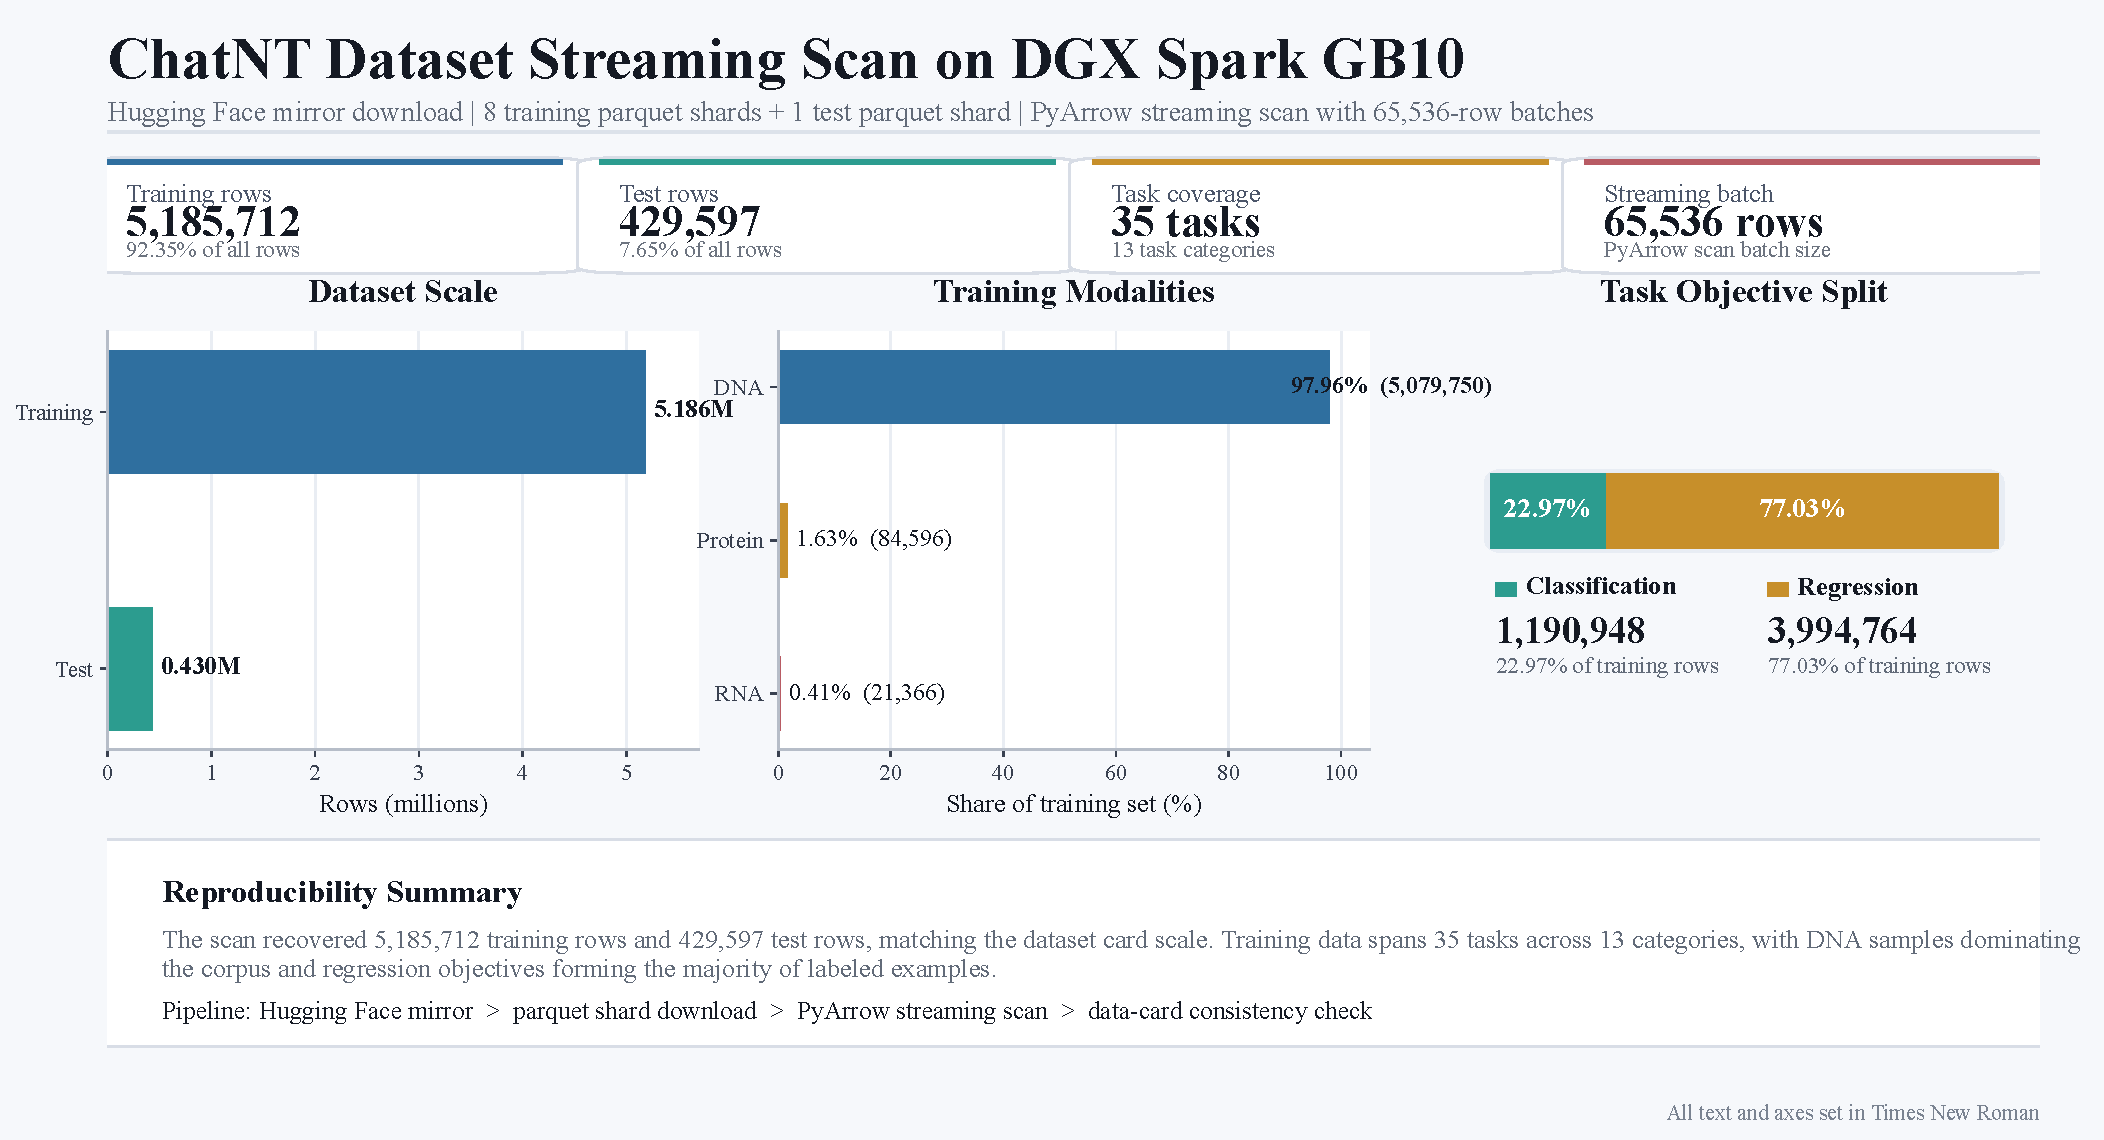
\includegraphics[width=0.95\linewidth]{./figs/chatnt_dgx_spark_dataset_profile.pdf}
    \caption{ChatNT 训练集和测试集样本分布}
\end{figure}

实验在 DGX Spark GB10 上完成，通过 Hugging Face 镜像下载 ChatNT 的 8 个训练 parquet 分片与 1 个测试 parquet 分片后，使用 PyArrow 按 65,536 行批大小进行流式扫描。训练集共 5,185,712 行，测试集共 429,597 行，与数据卡规模一致。训练集覆盖 35 个任务、13 个任务类别，其中 DNA 样本 5,079,750 条、蛋白样本 84,596 条、RNA 样本 21,366 条；分类样本 1,190,948 条，回归样本 3,994,764 条。

扫描吞吐为 35,265.7 行/秒，测试集扫描吞吐为 36,307.1 行/秒。训练集平均序列长度为 295.46，P50 为 205，P95 为 512，粗估计训练 token 平均值为 209.69，P50 为 175，P95 为 313。这说明 ChatNT 不是少量超长样本主导的数据集，而是由大量中短序列任务组成，真正的成本压力主要来自样本数和任务倾斜，而不是单条样本长度。

\begin{table}[H]
    \centering
    \renewcommand{\arraystretch}{1.2}
    \setlength{\tabcolsep}{20pt}
    \caption{ChatNT 数据集流式扫描吞吐与长度统计}
    \begin{tabular}{ccccc}
        \bottomrule[1.5pt]
        统计维度 & 指标 & 平均值/吞吐 & P50 & P95 \\
        \midrule[0.75pt]
        \multirow{2}{*}{扫描吞吐}
            & 训练集 & 35,265.7 行/秒 & -- & -- \\
            & 测试集 & 36,307.1 行/秒 & -- & -- \\
        \midrule[0.75pt]
        序列长度 & 训练集 & 295.46 & 205 & 512 \\
        粗估 token 成本 & 训练集 & 209.69 & 175 & 313 \\
        \toprule[1.5pt]
    \end{tabular}
\end{table}

\begin{figure}[H]
    \centering
    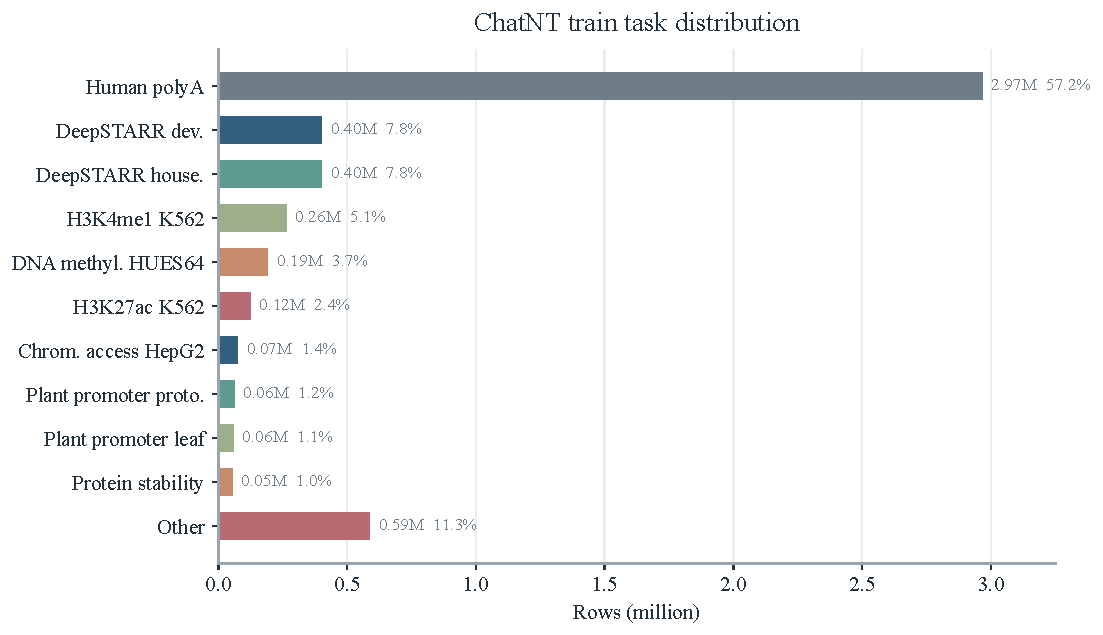
\includegraphics[width=0.95\linewidth]{./figs/task_distribution.pdf}
    \caption{ChatNT 训练集任务分布 human\_polya 单任务占 57.19\% 显示出明显头部倾斜}
\end{figure}

\begin{figure}[H]
    \centering
    \begin{minipage}[t]{0.6\linewidth}
        \centering
        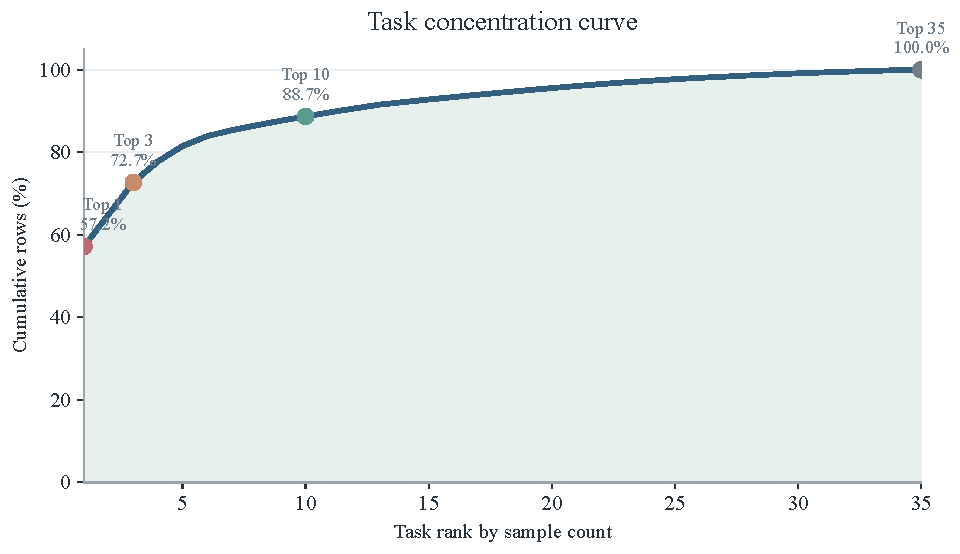
\includegraphics[width=\linewidth]{./figs/task_pareto.pdf}
        \caption{任务集中度 Pareto 曲线，前 1 个任务已占 57.2\%，前 10 个任务累计占 88.7\%}
    \end{minipage}
    \hfill
    \begin{minipage}[t]{0.35\linewidth}
        \centering
        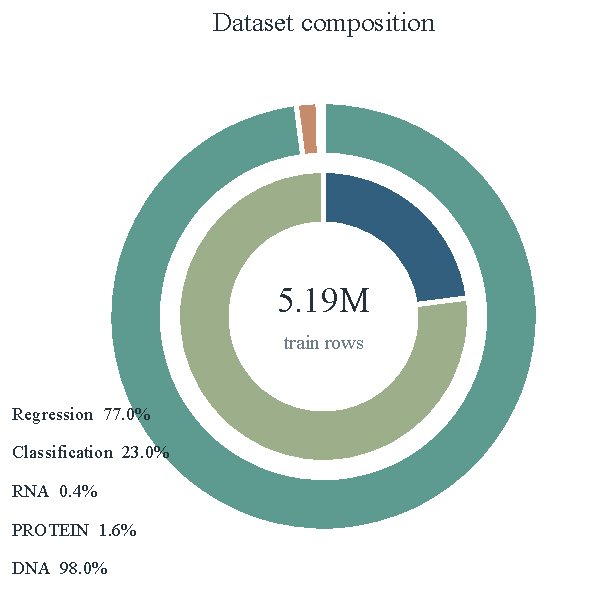
\includegraphics[width=\linewidth]{./figs/dataset_composition.pdf}
        \caption{训练集模态与任务类型构成，外环表示 DNA/RNA/蛋白模态，内环表示分类与回归}
    \end{minipage}
\end{figure}

\begin{figure}[H]
    \centering
    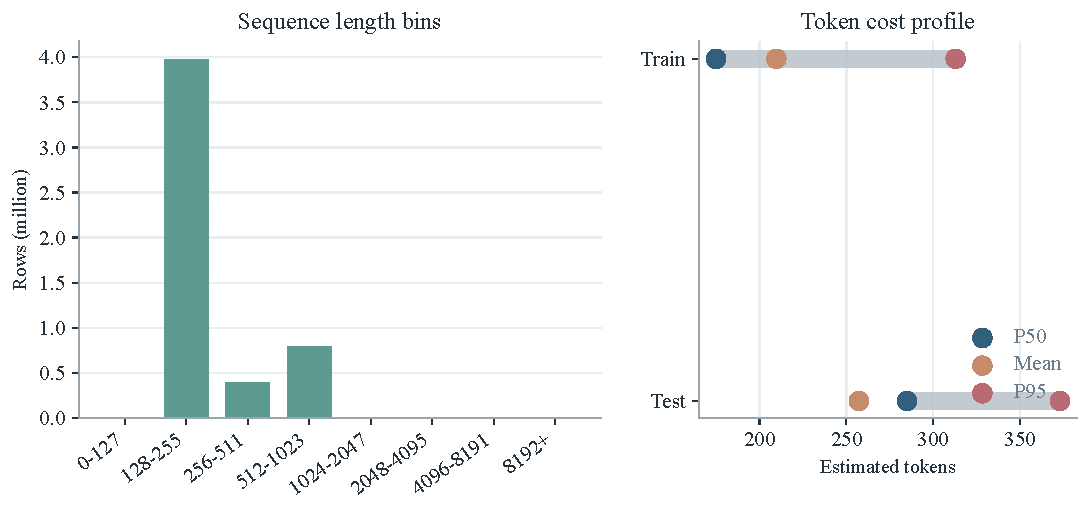
\includegraphics[width=0.95\linewidth]{./figs/length_token_distribution.pdf}
    \caption{训练集序列长度与粗估 token 成本分布，多数样本集中在 512 token 以下，适合先做样本选择再进入微调}
\end{figure}

任务分布见图 1，human\_polya 单任务达到 2,965,504 行，占训练集 57.19\%，deepstarr developmental 与 deepstarr housekeeping 各 402,034 行，分别占 7.75\%，而 protein stability、promoter、splice site、histone modification 等任务分散在长尾区域。Pareto 曲线进一步说明，前 3 个任务已经覆盖 72.7\% 的训练行，前 10 个任务覆盖 88.7\%，因此“随机抽样”并不等价于“多任务均衡抽样”。嵌套环图则说明，数据主体是 DNA 与回归任务，蛋白、RNA 和分类任务更需要在样本选择阶段获得显式保护，若直接随机采样，模型在训练预算内会大量重复学习头部任务，长尾任务很难获得足够覆盖。



\subsection{质量标记与重复分析}
我将硬风险与软风险分开处理，硬风险包括空字段、URL、邮箱、危险生物短语、非法 DNA 字符和极端 token 长度，软风险主要是 FASTA header 或坐标字段中的长数字串，因为这类数字常常是来源追踪或基因组坐标，不适合直接等同于个人隐私。

\begin{table}[H]
    \centering
    \renewcommand{\arraystretch}{1.2}
    \setlength{\tabcolsep}{24pt}
    \caption{训练集质量画像实测结果}
    \begin{tabular}{ccc}
        \toprule[1.5pt]
        指标 & 数值 & 解释 \\
        \midrule[0.75pt]
        训练样本数 & 5,185,712 & 8 个 parquet 分片合计 \\
        硬规则有效样本 & 5,180,604 & 有效率 99.90\% \\
        来源追踪软风险 & 2,711,970 & 长数字串命中率 52.30\% \\
        模板重复率 & 86.50\% & \texttt{exchanges} 模板大量复用 \\
        精确序列重复行 & 898,635 & 占训练集 17.33\% \\
        极端 token 粗估 & 5,108 & 占训练集 0.10\% \\
        \bottomrule[1.5pt]
    \end{tabular}
\end{table}

ChatNT 的格式质量整体较好：空字段、邮箱、URL、危险生物短语和非法 DNA 字符均未命中，极端 token 长度样本只有 5,108 条。更有价值的发现来自重复结构：训练集只有 699,921 个不同 \texttt{exchanges} 模板，模板重复率达到 86.50\%，精确序列重复行约 89.86 万，占 17.33\%。这里说明了对于 ChatNT，质量评估不应写成“清除脏数据”，而应聚焦“减少重复训练、提升长尾覆盖、控制来源泄漏”。

\begin{figure}[H]
    \centering
    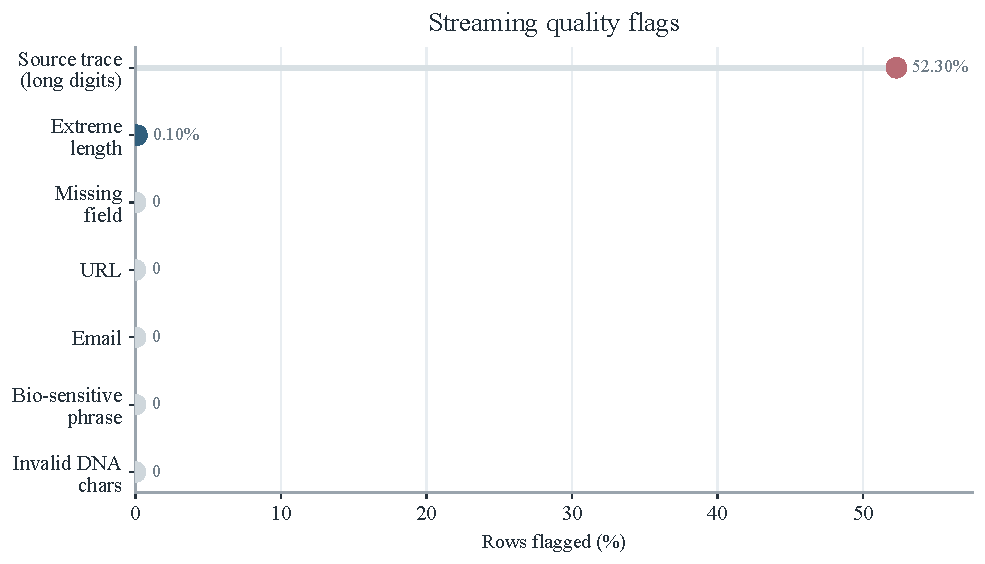
\includegraphics[width=0.87\linewidth]{./figs/quality_flags.pdf}
    \caption{流式质量标记统计，长数字串被作为来源追踪软风险处理，其他硬风险命中极少}
\end{figure}

\begin{figure}[H]
    \centering
    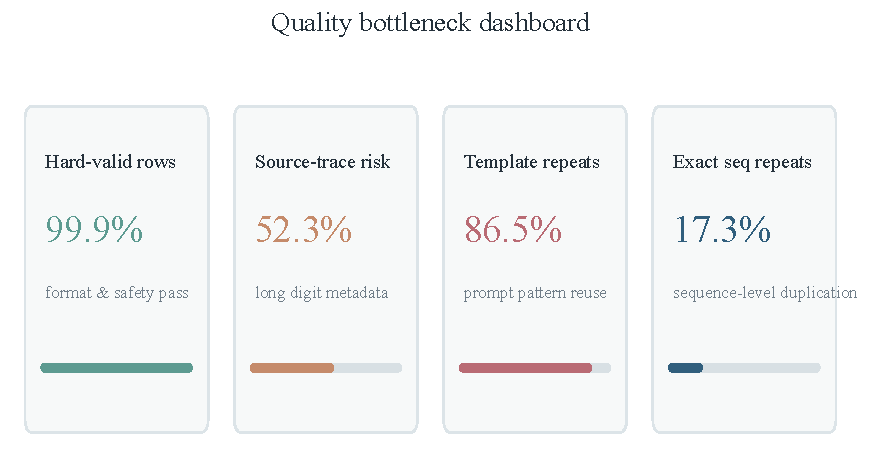
\includegraphics[width=0.95\linewidth]{./figs/quality_bottleneck_dashboard.pdf}
    \caption{质量瓶颈仪表盘，硬格式有效率很高，但来源追踪、模板重复与序列重复构成主要优化空间}
\end{figure}

质量瓶颈仪表盘把表格中的数值拆成四类决策信号：硬规则有效率达到 99.9\%，说明继续堆叠普通清洗规则的边际收益有限，来源追踪软风险达到 52.3\%，提示需要在保留科学信息和避免记忆来源标识之间做更细的脱敏策略，模板重复率 86.5\%、精确序列重复率 17.3\%，则直接对应微调阶段的预算浪费问题。因此，本文后续策略把重点放在“去重复倾斜”和“保留长尾覆盖”，而不是把数据集简单描述为脏数据清洗任务。



\subsection{Zig 流式扫描基准}
为了验证系统级流式处理能力，本文从训练集导出 200,000 行 JSONL 样本，文件大小 214.05MB，并使用 Zig 0.16.0 编译 ReleaseFast 扫描器统计行数、字节数与长数字 run，扫描器通过 1MB 缓冲区从标准输入读取，不需要加载完整文件。

\begin{table}[htbp]
    \centering
    \renewcommand{\arraystretch}{1.2}
    \setlength{\tabcolsep}{30pt}
    \caption{Zig JSONL 流式扫描基准}
    \begin{tabular}{ccc}
        \toprule[1.5pt]
        指标 & 数值 & 备注 \\
        \midrule[0.75pt]
        JSONL 行数 & 200,000 & 从训练集导出 \\
        文件大小 & 214.05MB & UTF-8 JSONL \\
        扫描耗时 & 0.17s & \texttt{/usr/bin/time} 计时 \\
        吞吐 & 1,176,470 行/s & 单进程流式读取 \\
        字节吞吐 & 1,259.09 MB/s & ReleaseFast 编译 \\
        峰值 RSS & 1,496KB & 约 1.5MB \\
        \bottomrule[1.5pt]
    \end{tabular}
\end{table}

该结果说明 Zig 适合承担论文中“靠近原始数据的一线扫描器”角色。相比把全量 JSONL 交给 Python 逐行解析，Zig 可以先以极低内存成本完成行级过滤、风险粗标和统计摘要，再把结构化 meta 输出给后续列式分析层。



\subsection{Qwen3.6 Tokenizer 校准}
token 成本不能只按字符数主观估计，我们从训练集中抽取 8,000 条样本，调用本地 Qwen3.6-27B Tokenizer 计算真实 token 数，并用 \texttt{exchange\_chars} 与 \texttt{seq\_len} 拟合线性估计器，拟合结果为：
\begin{align}
    \widehat{\mathrm{tokens}}=0.001+0.2389\cdot\mathrm{exchange\_chars}+0.5124\cdot\mathrm{seq\_len}
\end{align}

线性估计器的平均绝对误差为 4.66 token，而原始粗估计的平均绝对误差为 29.17 token，由于样本长度高度集中，整体 $R^2$ 只有 0.323，但误差规模已经足以支持预算级样本选择，不逐条调用 Tokenizer 的情况下，快速剔除极端长度样本，并对边界样本再做精确复核。

\begin{figure}[H]
    \centering
    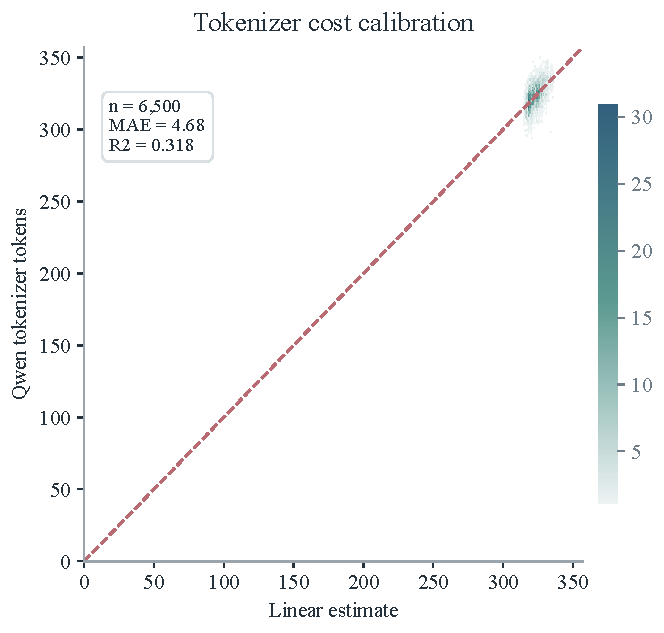
\includegraphics[width=0.66\linewidth]{./figs/token_calibration.pdf}
    \caption{Qwen3.6 Tokenizer 校准抽样 8,000 条样本，线性估计器 MAE 为 4.66 token}
\end{figure}



\subsection{样本选择策略对比}
最后，本文在 260,000 条固定种子 reservoir 样本上模拟 300 万 token 预算下的数据选择，四种策略分别为 Random、Clean-only、Quality-top 和 Diversity-balanced。Quality-top 直接选择质量分最高样本，Diversity-balanced 则在质量分排序基础上进行任务轮转，防止头部任务吞掉预算。

\begin{table}[H]
    \centering
    \renewcommand{\arraystretch}{1.2}
    \setlength{\tabcolsep}{8pt}
    \caption{300 万 token 预算下的数据选择模拟}
    \begin{tabular}{cccccc}
        \toprule[1.5pt]
        策略 & 样本数 & 任务覆盖 & 类别覆盖 & 任务熵 & 头部任务占比 \\
        \midrule[0.75pt]
        Random & 14,332 & 35 & 13 & 0.528 & 57.30\% \\
        Clean-only & 14,457 & 35 & 13 & 0.527 & 57.31\% \\
        Quality-top & 8,513 & 14 & 8 & 0.948 & 14.88\% \\
        Diversity-balanced & 9,759 & 35 & 13 & 1.000 & 2.86\% \\
        \bottomrule[1.5pt]
    \end{tabular}
\end{table}

结果表明，Clean-only 与 Random 几乎没有拉开差距，这是因为 ChatNT 的硬格式风险本来就很低，真正的问题是头部任务倾斜。Quality-top 能显著降低来源追踪软风险并提高平均质量分，但只覆盖 14 个任务和 8 个类别，可能牺牲长尾能力。

\begin{figure}[H]
    \centering
    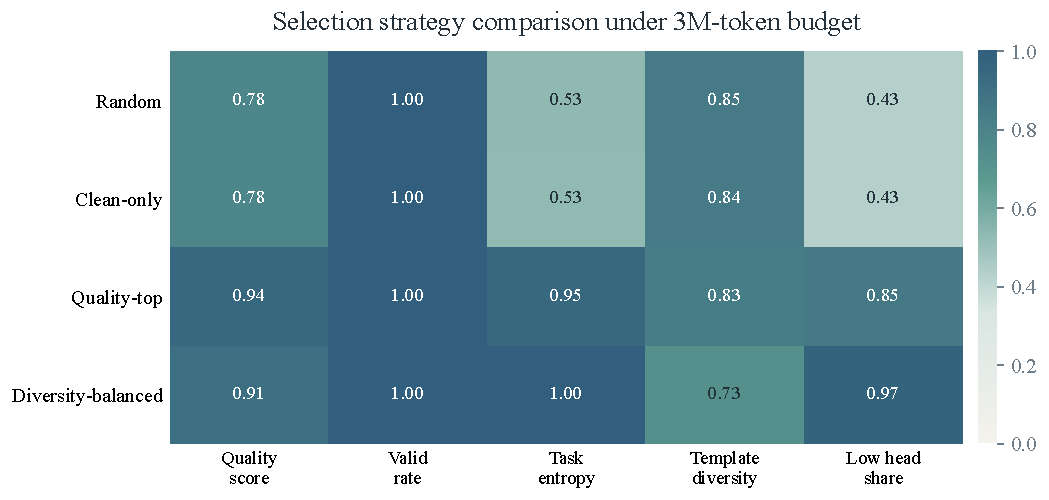
\includegraphics[width=0.95\linewidth]{./figs/selection_comparison.pdf}
    \caption{相同 token 预算下的样本选择策略对比，Diversity-balanced 在保持硬规则有效率的同时显著提升任务均衡性}
\end{figure}

样本选择前沿图更直观地展示了这个取舍：Quality-top 位于高质量区域，但气泡较小，说明任务覆盖不足，Diversity-balanced 在质量分略低的情况下获得最高任务熵和最大任务覆盖，是更接近 Pareto 最优的策略。类别预算分配图进一步说明，Random 会把大部分 token 花在 polyA 与少数头部类别上，而 Diversity-balanced 将预算重新分散到 histone、RNA degradation、splice site、protein fitness、promoter 等类别。Diversity-balanced 覆盖全部 35 个任务和 13 个类别，将头部任务占比降到 2.86\%，任务熵接近 1.000，是更适合多任务生物序列微调的选择策略。这个结果把论文核心观点从“清洗能提升质量”推进到“质量评分必须与覆盖约束共同使用”。

\begin{figure}[H]
    \centering
    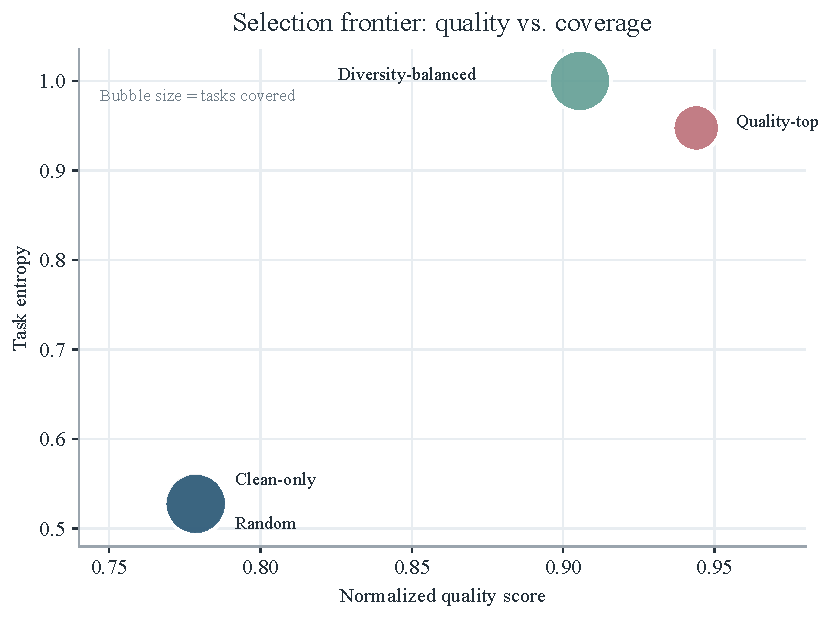
\includegraphics[width=0.65\linewidth]{./figs/selection_frontier.pdf}
    \caption{横轴为归一化质量分，纵轴为任务熵，气泡大小表示覆盖任务数}
\end{figure}

\begin{figure}[H]
    \centering
    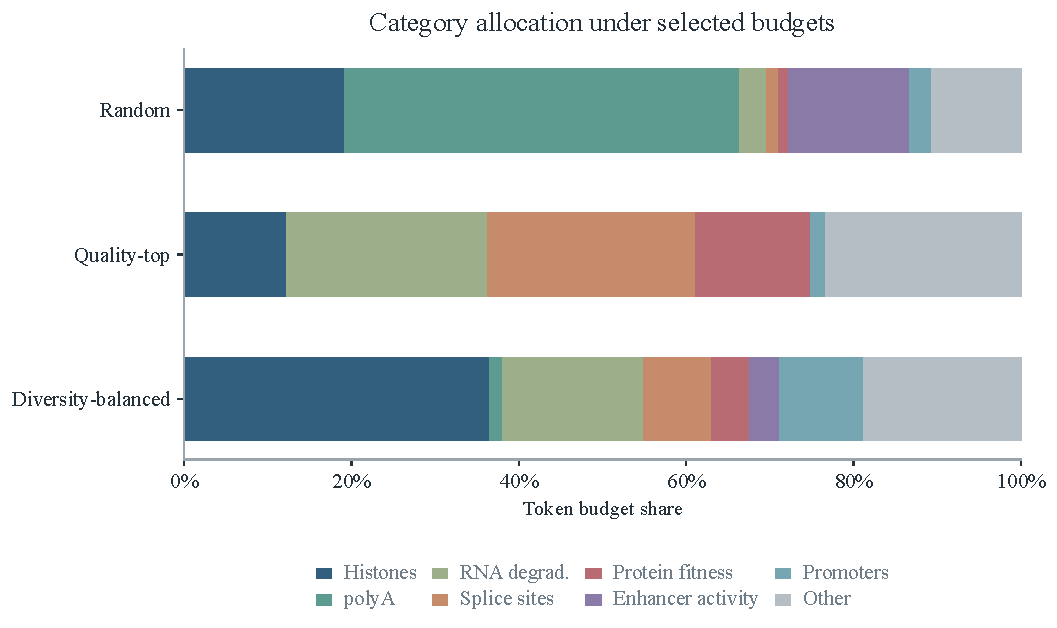
\includegraphics[width=0.85\linewidth]{./figs/category_allocation.pdf}
    \caption{堆叠条形展示 300 万 token 被各任务类别消耗的比例}
\end{figure}



\section{创新性}

\begin{itemize}
    \item 第一个创新是提出“训练价值驱动”的数据质量定义，传统清洗把目标停留在删除坏样本，本文进一步追问样本是否对当前基座模型有学习价值。通过把 Loss、遗忘、增益和推理稳定性写回，样本质量从静态分数变为可迭代更新的动态属性。
    \item 本文的第二个创新是将 Zig 与 Polars 组合用于大模型微调数据工程，Zig 负责 JSONL 一线流式扫描，适合低内存、高吞吐、可静态编译的场景，Polars 负责列式聚合、惰性优化、分层采样和报告生成，这种组合比单一 Python 脚本更能体现大数据系统设计，也更贴合“流式解析、文本清洗、去重、敏感词扫描、token 粗估计、PII 脱敏”和“Rust/Polars 流水线”。
    \item 第三个是选择生物序列指令数据作为微调质量评估对象，DNA/RNA/蛋白序列不是普通文本，序列相似、任务一致性、标签合法性、长上下文截断和生物安全风险都更复杂，用 ChatNT 做研究设想，可以让论文从通用聊天清洗走向更有科学问题感的“生物序列大数据如何塑造模型能力”。
    \item 最后一个创新是把训练、部署、数据评估连接起来，我不只讨论离线质量分，而且设计从 parquet 到 JSONL、从 Zig 扫描到 Polars 质量表、从 LoRA Adapter 到 vLLM 服务、从推理评测到反馈回写的闭环。
\end{itemize}



\section{可能存在的技术困难与瓶颈}

\begin{itemize}
    \item[$\divideontimes$] 生物学正确性难以完全自动验证，格式正确并不代表标签正确，启动子、剪接位点、组蛋白修饰、RNA 降解和蛋白性质预测都有各自实验背景，仅靠通用规则无法判断答案是否科学，因此如果后续我做实验，需要为高价值任务设计任务专用验证器，并对高风险簇进行人工抽样复核。
    \item[$\divideontimes$] 近似去重可能误伤有价值样本，两个 DNA 序列 k-mer 相似并不必然表示任务重复，两个问题模版相似也不代表答案冗余，SimHash 与 MinHash 应被用于发现候选重复簇，而不是直接做硬删除，真正的样本保留决策还应结合任务、标签、长度、训练反馈和人工审计。
    \item[$\divideontimes$] 训练反馈本身有计算成本，若对 500 多万条样本逐条计算样本级 Loss 或梯度冲突，成本可能超过训练节省，可行方案是先按任务、长度和重复簇分层抽样，计算簇级反馈，再将权重传播给同簇样本，对边界、高风险和长尾任务样本再做精细反馈。
    \item[$\divideontimes$] 长上下文能力与显存预算存在矛盾，Qwen3.6-27B 的配置支持很长位置编码，但 LoRA 训练时仍受显存、batch size、attention 实现和吞吐限制，简单截断 DNA 序列可能破坏远距离依赖，完全保留又会浪费大量 token，后续需要研究任务感知截断、滑窗摘要、重要区域抽取和多视图训练。
\end{itemize}



\section{结论}
本文以 ChatNT 生物序列指令数据和 Qwen3.6-27B 权重基础，研究了“面向生物序列大数据微调大模型的质量评估”问题，本文的核心结论是：领域大模型微调的关键不只是训练脚本，而是数据质量的系统化度量、预算约束下的样本选择，以及未来可接入训练反馈的闭环优化。

实测结果表明，ChatNT 训练集规模达到 5,185,712 条，格式硬风险很低，硬规则有效率为 99.90\%，但其模板重复率达到 86.50\%，精确序列重复行占 17.33\%，human\_polya 单任务占比达到 57.19\%。这说明该数据集的主要质量瓶颈不是“脏数据太多”，而是“重复、倾斜和预算浪费”，Zig 流式扫描在 214MB JSONL 样本上达到 1.26GB/s、约 117.6 万行/s，峰值内存约 1.5MB，证明系统级扫描器适合作为大数据质量流水线的第一层。Qwen3.6 Tokenizer 校准将 token 估计 MAE 从 29.17 降至 4.66，为低成本 token 预算控制提供了依据。在 300 万 token 预算模拟中，Diversity-balanced 策略覆盖全部 35 个任务和 13 个类别，并把头部任务占比从随机采样的 57.30\% 降至 2.86\%。

因此，本文不仅提出了从 parquet 到 JSONL、从 Zig 扫描到列式画像、从质量评分到分层样本选择、从 LoRA/vLLM 到反馈回写的闭环路线，也通过实测数据验证了微调前数据质量评估的必要性。后续工作可在八卡 A6000 等更强训练环境中接入 LoRA 样本级 Loss、验证集增益和推理稳定性信号，使本文的数据侧质量分真正演化为“数据特征 - 训练动态 - 模型能力”的闭环优化系统。



\begin{thebibliography}{32}
    \bibitem{chatnt_dataset}
    InstaDeepAI.
    \newblock Dataset Card for ChatNT Training Data.
    \newblock 2025.
    \newblock \url{https://huggingface.co/datasets/InstaDeepAI/ChatNT_training_data}

    \bibitem{qwen36}
    Qwen Team.
    \newblock Qwen3.6-27B: Flagship-Level Coding in a 27B Dense Model.
    \newblock 2026.
    \newblock \url{https://huggingface.co/Qwen/Qwen3.6-27B}

    \bibitem{lora}
    Edward J. Hu, Yelong Shen, Phillip Wallis, Zeyuan Allen-Zhu, Yuanzhi Li, Shean Wang, Lu Wang, and Weizhu Chen.
    \newblock LoRA: Low-Rank Adaptation of Large Language Models.
    \newblock 2021.
    \newblock \url{https://arxiv.org/abs/2106.09685}

    \bibitem{qlora}
    Tim Dettmers, Artidoro Pagnoni, Ari Holtzman, and Luke Zettlemoyer.
    \newblock QLoRA: Efficient Finetuning of Quantized LLMs.
    \newblock 2023.
    \newblock \url{https://arxiv.org/abs/2305.14314}

    \bibitem{zig016}
    Zig Software Foundation.
    \newblock Zig 0.16.0 Release Notes.
    \newblock 2026.
    \newblock \url{https://ziglang.org/download/0.16.0/release-notes.html}

    \bibitem{polars_lazy}
    Polars.
    \newblock Lazy API, Polars User Guide.
    \newblock \url{https://docs.pola.rs/user-guide/lazy/using/}

    \bibitem{polars_streaming}
    Polars.
    \newblock Streaming, Polars User Guide.
    \newblock \url{https://docs.pola.rs/user-guide/concepts/streaming/}

    \bibitem{vllm}
    Woosuk Kwon, Zhuohan Li, Siyuan Zhuang, Ying Sheng, Lianmin Zheng, Cody Hao Yu, Joseph E. Gonzalez, Hao Zhang, and Ion Stoica.
    \newblock Efficient Memory Management for Large Language Model Serving with PagedAttention.
    \newblock \emph{Proceedings of SOSP}, 2023.
    \newblock \url{https://arxiv.org/abs/2309.06180}
\end{thebibliography}



\end{document}
